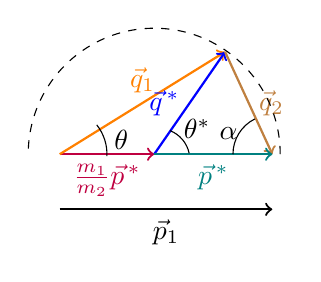
\begin{tikzpicture}
\draw [->, thick, purple](-1.2,-0.5) node (v1) {} -- (0,-0.5) node [midway, below] {$\frac{m_1}{m_2}\vec{p}^{\,*}$};
\draw [->, thick, orange] (v1.center) -- (0.9,0.8) node [midway, above] {$\vec{q}_1$};
\draw [->, thick, blue](0,-0.5) node (v3) {} -- (0.9,0.8)node [midway, left] {$\vec{q}^{\,*}$};
\draw [->, thick, brown] (0.9,0.8) -- (1.5,-0.5) node [midway, right] {$\vec{q}_2$};
\draw[->, thick, teal] (v3.center) -- (1.5,-0.5)node [midway, below] {$\vec{p}^{\,*}$};
\draw [->, thick](-1.2,-1.2) -- (1.5,-1.2)node [midway,below] {$\vec{p}_1$};

\draw (0.2,-0.2) arc (68.4061:12:0.4)node [midway, above right=-3] {$\theta^*$};
\draw (1,-0.5) arc (180:116.4:0.5)node [midway, left=-3] {$\alpha$};
\draw [dashed] (1.6,-0.5) arc (0:180:1.6);
\draw (-0.6005,-0.5251) arc (-2.3975:38.4:0.6)node [midway, right] {$\theta$};
%\node at (-0.9,1.5) {$m_1<m_2$};
\end{tikzpicture}